

This chapter introduces machine learning architectures or layers that are used in this work, specifically Long Short Term Memory Networks (LSTM) Temporal Convolutional Networks (TCN) and Transformers. These are all architectures usually used for sequential data. Finally, we define types of errors in researching a machine learning model. 

\hfill \break

Machine learning has become key to important applications in science, technology and commerce. The focus of machine learning is on the problem of prediction: given a sample of training examples $(x_1,y_1),...,(x_n,y_n) \in \mathbb{R}^d \times \mathbb{R}^p$ we learn a predictor $h_n: \mathbb{R}^d \rightarrow \mathbb{R}^p$ that is used to predict the label $y$ of a new point $x$, unseen in training.

\hfill \break

The prediction $h_n$ is commonly chosen from some function class $H$, such as neural networks with a certain architecture, using empirical risk minimization (ERM) and its variants. We can see neural network as function class because neural networks model functions and by changing their weight we parametrize over a function space.  In ERM, the predictor is taken to be a function $h \in H$ that minimizes the empirical (or training) risk: $$\frac{1}{n} \sum_{i=1}^n l(h(x_i),y_i)$$
where $l$ is a loss function, such as the squared loss $l(y',y)=(y'-y)^2$ for regression or 0-1 loss $l(y',y)=1_{\{y' \neq y\}}$ for classification.

\hfill \break

The goal of machine learning is to find $h_n$ that performs well on new data, unseen in training. To study performance on new data, knows as generalization, we typically assure the training example are sampled randomly from a probability distribution $P$ over $\mathbb{R}^d \times \mathbb{R}$ and evaluate $h_n$ on a new test example $(x,y)$ drawn independently from $P$. The challenge arises from the mismatch between the goals of minimizing the empirical risk, the explicit goal of ERM algorithms i.e. optimization, and minimizing the true (or test) risk:
$$\EX_{(x,y) \sim P}[\ell (h(x),y)]$$
the goal of machine learning.

\section{Sequence modeling task}
Before defining network architectures, we define the nature of the sequence modeling task. Suppose that we are given an input sequence $x_1,...,x_N$ and wish to predict some corresponding output $y_1,...,y_N$ at each time. The key constraint is that to predict the output $y_t$ for some time $t$, we are constrained to only use those inputs that have previously observed: $x_1,...,x_t$. Formally, a sequence modeling network is any function $f:X^t \rightarrow Y^t$ that produces the mapping:
$$\hat{y}_1,...,\hat{y}_N = f(x_1,...,x_N)$$
if it satisfies the causal constraint that $y_t$ depends only on $x_1,...,x_t$ and not on any future inputs $x_{t+1},...,x_N$. The goal of learning, in the sequence modelling setting, is to find a network $f$ that minimizes some expected loss between the actual outputs and the predictions $L(y_1,...,y_N,f(x_1,...,x_N))$, where the sequences and outputs are drawn according to some distribution.
This formalism covers many contexts such as auto-regressive prediction, where we try to predict some signal given its past, by setting the target output to be simply the input shifted by one time step. This formalism does not, however, directly capture domains such as machine translation, on sequence-to-sequence prediction in general, since in these cases the entire input sequence including future states can be needed to predict the output.

\section{Recurrent neural network}
The recurrent neural network (RNN) architecture was introduce by Rumelhart et al. \cite{rumelhart1986learning} in 1986. RNNs operate on sequence of data by applying an identical function $f$ to every element of the sequence to produce a sequence of state vectors $H = [h_1,...,h_p]$. The function $f$ takes as input both the output of the function at the previous point in the sequence, and the current element of the input sequence $X=[x_1,...,x_p]$. An RNN can be unfolded to represent it as a traditional feedforward neural network with no recurrence. A generic RNN is shown in figure \ref{fig:generic_rnn}.

\begin{figure}[h]
    \centering
    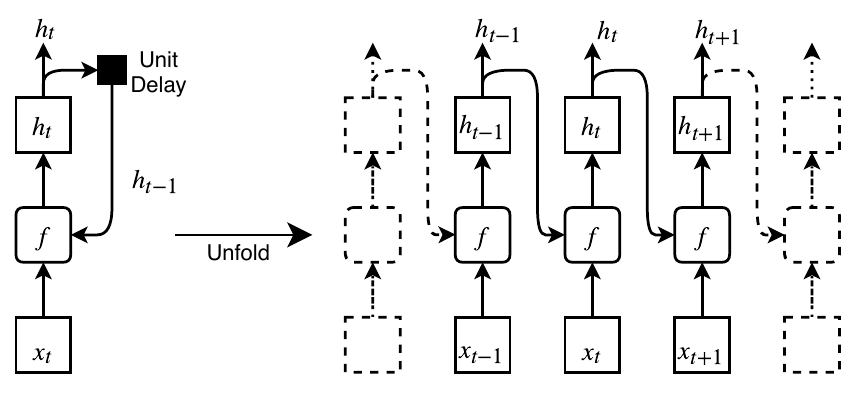
\includegraphics[width=10cm]{cap3/generic_rnn.png}
    \caption{Generic recurrent neural network}
    \label{fig:generic_rnn}
\end{figure}

At each point $t$ in the sequence $h_t$ is taken as the output. $h_t$ can be projected to the required output dimension for example with a dense layer. 

\hfill \break

\begin{figure}[h]
    \centering
    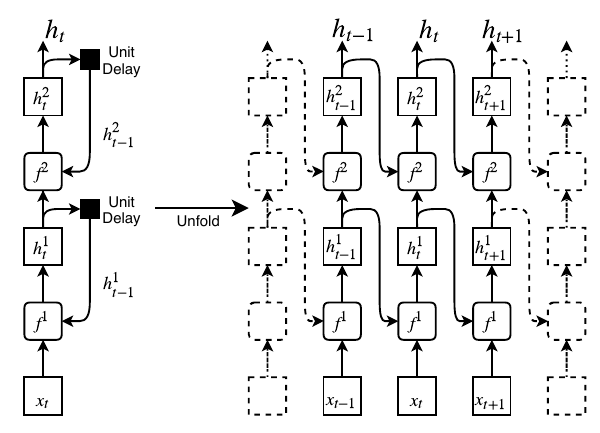
\includegraphics[width=10cm]{cap3/two_layer_rnn.png}
    \caption{Two-layer recurrent neural network}
    \label{fig:two_layer_rnn}
\end{figure}

RNNs can be extended to multiple layers, with a two-layer RNN illustrated in figure \ref{fig:two_layer_rnn}. Each layer implements its own function, with layer $n$ implementing function $f^n$ and producing output $h^n$. For layers after the first layer, instead of taking a $x$ vector as input they take the state vector from the previous layer. There can be an arbitrary number of layers. A multi-layer RNN can in fact be thought as a generalization of a single-layer, where multiple sub-function are included in the function $f$.


\subsection{Long Short Term Memory Network}
\label{lstm_section}
Recurrent networks are often used in sequence processing tasks because of their ability to capture temporal relationships. Long Short Term Memory (LSTM) is a modified version of recurrent neural networks proposed by Hochreiter and Schmidhuber \cite{longshortterm}. Moreover, Recurrent Neural Networks are prone to vanishing and exploding gradients problems \cite{goodfellow2016deep}, which can be addressed through the use of long short term memory cell. An LSTM cell is able to selectively add and remove elements from the state vector as it passes through the cell. LSTM cells have been demonstrated to outperform simpler functions in a variety of tasks when employed as RNN function \cite{chung2014empirical} \cite{jozefowicz2015empirical} \cite{le2015simple}. The LSTM cell extends the standard RNN model by separating the cell output $c_t$ from the cell state $h_t$, shown in figure \ref{fig:lstm_cell} and its multi-layer configuration shown in figure \ref{fig:multilayer_lstm}. The LSTM cell is described by the following equations:

\begin{align}
    f_t & = \sigma(W_f x_t + U_f h_{t-1} + b_f) \label{lstm_eq_begin}\\
    i_t & = \sigma(W_i x_t + U_i h_{t-1} + b_i) \\
    o_t & = \sigma(W_o x_t + U_o h_{t-1} + b_o) \\
    \hat{c_t} & = \tanh(W_c x_t + U_c h_{t-1} + b_c) \\
    c_t & = f_t \circ c_{t-1} + i_t + \hat{c_t} \\
    h_t & = o_t \circ \tanh(c_t) \label{lstm_eq_end}
\end{align}

where:
\begin{itemize}
    \item $\circ$ denotes the element-wise multiplication:
    \item the input vector is $x_t \in \mathbb{R}^n$
    \item the cell output vector is $h_t \in \mathbb{R}^d$ ($d$ is the hidden dimension of the model);
    \item the cell state vector is $c_t \in \mathbb{R}^d$;
    \item the forget gate vector is $f_t \in \mathbb{R}^d$;
    \item the input gate vector is $i_t \in \mathbb{R}^d$
    \item the output gate vector is $o_t \in \mathbb{R}^d$
    \item the cell candidate vector is $\hat{c_t} \in \mathbb{R^d}$;
    \item the learned cell state weight matrices are $U \in \mathbb{R}^{d \times N}$;
    \item the learned input weight matrices are $W \in \mathbb{R}^{d \times d}$
    \item the learned bias vectors $b \in \mathbb{R^d}$; and
    \item $\sigma(y)=\frac{1}{1+e^{-y}}$ represents the sigmoid function
\end{itemize}

At first glance equations \ref{lstm_eq_begin} to \ref{lstm_eq_end} may come across difficult, but they are in fact highly intuitive when studied alongside figure \ref{fig:lstm_cell}. There are three primary sub-sections within the LSTM cell, discussed in the three following paragraphs. Note that the use of two weight matrices (W and U) in the LSTM equations is equivalent to concatenating $x$ and $h$ and using a single weight matrix - keeping consistency with figure \ref{fig:lstm_cell}. 

\hfill \break

First, data is removed from the cell state (c) as it flows through the LSTM cell. The sigmoid function that produces $f_t$ outputs values between 0 and 1. When these are multiplied with $c_{t-1}$ (the previous cell state) some elements will be removed or reduced. The sigmoid layer that produces $f_t$ is referred to as the \textit{forget gate}, as it causes some data to be removed from the cell state depending on the previous cell output ($h_{t-1}$) and the current input ($x_t$).

\hfill \break

Next, information is added to the cell state. The $\tanh$ layer produces a new candidate cell state ($\hat{c_t}$), and the input gate layer produces $i_t$ in a similar fashion to $f_t$. The vector $i_t$ decides which elements of the new candidate cell state vector are added to the actual cell state vector by reducing the magnitude of elements in $\hat{c_t}$ based on the previous cell output ($h_{t-1}$) and the current input ($x_t$). After $\hat{c_t}$ has been multiplied by $i_t$ to selectively reduce elements it is added to the cell state. The sigmoid layer that produces $i_t$ is referred to as the input gate, as it decides what data is added to the cell state as it passes through the cell.

\hfill \break

Finally, a candidate output vector is produced by applying $\tanh$ element-wise to the cell state. The output gate layer produces $o_t$ and this is multiplied with the candidate output vector to selectively remove elements, producing the final cell output $h_t$. The sigmoid layer that produces $o_t$ is referred to as the output gate, as it decides which elements of the candidate output are passed as the final output.

\hfill \break

Together, these gating mechanism allow the LSTM cell to selectively add and remove elements from the state as it passes through the cell, and allow the cell to selectively produce an output based on the current cell state. This generally allows the LSTM cell to retain data from many timestep in the past, making it a superior choice to simpler functions when working with long sequences of data, though in some cases the LSTM cell can discard data from early in the sequence.


\begin{figure}[h]
    \centering
    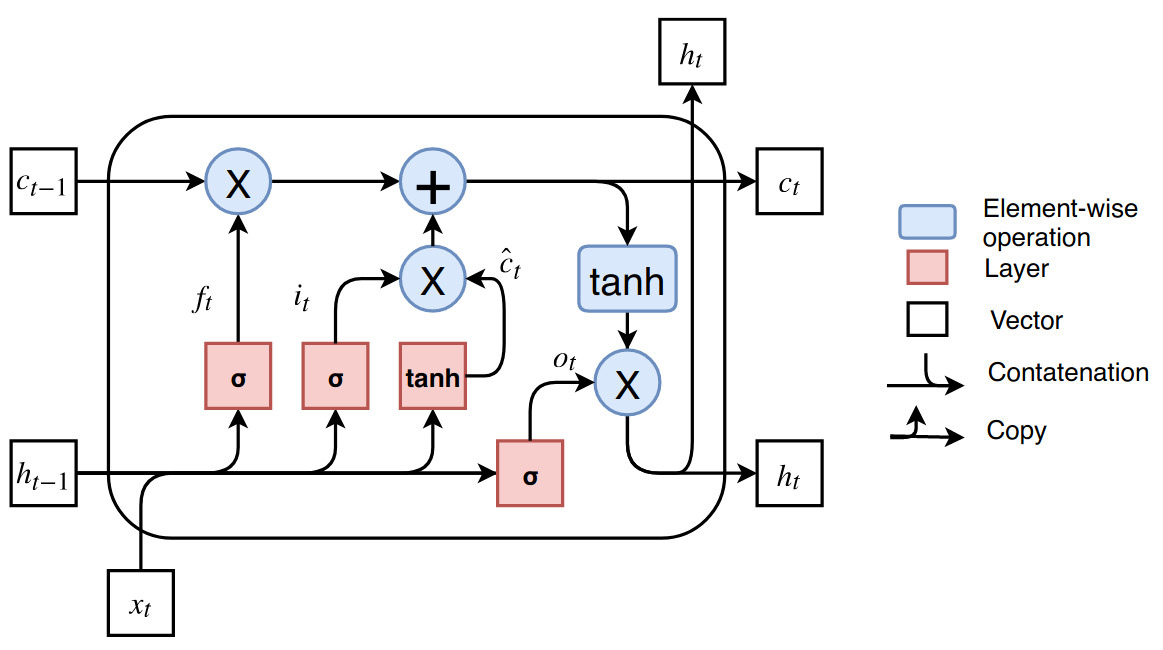
\includegraphics[width=10cm]{cap3/long-short-term-memory-cell.png}
    \caption{Long short-term memory cell.}
    \label{fig:lstm_cell}
\end{figure}

\begin{figure}[h]
    \centering
    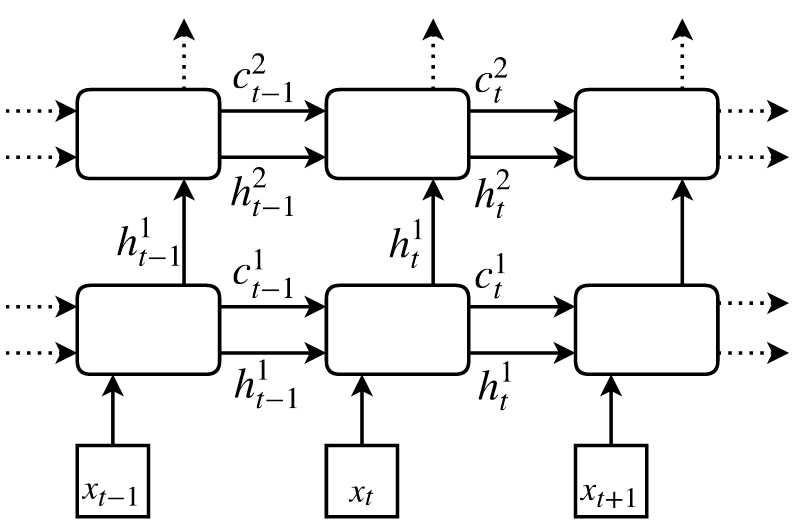
\includegraphics[width=10cm]{cap3/multi-layer long short term memory cell configuration.png}
    \caption{Multi-layer long short-term memory cell configuration.}
    \label{fig:multilayer_lstm}
\end{figure}

\section{Temporal Convolutional Networks}
\label{tcn_section}

Temporal Convolutional Networks were introduced in 2016 by Lea et al. \cite{lea2016temporal}. TCNs are one-dimensional causal dilated Convolutional Neural Network. In this section we define TCNs that will satisfy the following properties: (1) computations are performed layer-wise, meaning every time step is updated simultaneously, instead of updating sequentially per-sample (2) convolutions are computed across time, (3) prediction at each step are a function of a fixed-length period of time, which is referred to as the receptive field (4) the convolutions in the architecture are causal, meaning that there in no information leakage from future to past (5) the architecture can take a sequence of any length and map it to an output sequence of any length, just as with an RNN. We will show how TCNs can build very long effective history sizes (i.e. the ability for the network to look very far into the past to make a prediction) using a combination of very deep networks, augmented with residual layers, and dilated convolutions.
Figure \ref{fig:tcn} illustrates an example of Temporal Convolutional Network. TCN tends to be superior in many task to LSTM and also Bidirectional LSTM \cite{bidirectional_lstm}.

\subsection{Temporal convolution}

Let $X_t \in \mathbb{R}^{F_0}$ be the input feature vector of length $F_0$ for time step $t$ for $1 \leq t \leq T$. A TCN consist of $L$ layers denoted by $E^{(l)} \in \mathbb{R}^{F_l \times T_l}$ for $1 \leq l \leq L$ where $F_l$ is the number of convolutional filters in the $l-$th layer and $T_l$ is the number of corresponding time steps.
We define the collection of filters in each layer as $W=\{W^{(i)}\}^{F_l}_{i=1}$ for $W^{(i)} \in \mathbb{R}^d \times F_{l-1}$ with a corresponding bias vector $b \in R^{F_l}$. Given the signal from the previous layer, $E^{(l-1)}$, we compute activations $E^{(l)}$ with
$$ E^{(l)} = f(W * E^{(l-1)}+b) $$
where $f$ is the activation function and $*$ is the convolution operator. 

\subsection{Dilated causal convolution}

When dealing with Convolutional Neural Networks (CNNs), \textit{causal} means that each output $y_t$ of the network is exclusively a function of previous input timestep $x_0, ..., x_t$, while \textit{dilated} means that each hidden layer is given a \textit{dilatation factor} $d$ which controls which timestep from the previous layer the convolution is actually applied over. 
A simple causal convolution is only able to look back at history with size linear in the depth of the network. This makes it challenging to apply the before mentioned causal convolution on sequence tasks, especially those requiring longer history. The solution here is to employ dilated convolutions that enable an exponentially large receptive field. 
Given a sequence $x=x_0, ..., x_n \in \mathbb{R}$ and a filter $f: 0, ..., k-1 \rightarrow \mathbb{R}$, the \textit{dilated causal convolution} operation $x*_d f$ on the $t$-th element of $x$ is defined as follows:
$$(x*_d f)(t)=\sum\limits_{t=0}^{k-1} f(i) \cdot x_{t-d \cdot i} $$

where $d$ is the dilation factor, $k$ is the filter size, and $s-d \cdot i$ accounts for the direction of the past.
Note how $t-d \cdot i$ enforces the \textit{causal} part of the convolution, as it can only point to sequence elements which are in the past. Dilation is equalent to introducing a fixed step between every two adjacent filter step. When $d=1$, a dilated convolution reduces to a regular convolution. The dilatation factor $d$ usually increases the further we get into the network, often taking the values of increasing powers of two (i.e. $d=2^i$ on the $i$-th hidden layer of the network). This ensures two things. First, that the receptive field of the network grows exponentially with the number of layers (whereas in a undilated CNN this would grow linearly) granting a longer history. Second, that the output $y_t$ at time $t$ is effectively a function of a contiguous number of steps in the input. A network with $m$ layers has a receptive field of size $2^{m-1}k$. Therefore there are two ways to increase the receptive filed of the TCN, choosing a larger filter size $k$ and increasing the dilation factor $d$.

\subsection{Residual connections}
A residual block (He et al. 2016) \cite{residual_connections} contains a connection leading out to a series of transformations $F$, whose outputs are added to the input $x$ of the block.
$$ o = Activation(x+F(x))$$

This effectively allows layers to learn modifications to the identity mapping rather than the entire transformation, which has repeatedly been shown to benefit very deep networks.

\hfill \break

Since a TCN's receptive filed depends on the network depth $n$ as well as filters size $k$ and dilation factor $d$, stabilization of deeper and larger TCNs becomes important. For example, in a case where the prediction could depend on a history of size $2^{12}$ and a high-dimensional input sequenced, a network of up to 12 layers could be needed. Each layer, more specifically, consists of multiple filters for feature extraction. 

\hfill \break

However, whereas in a standard Residual Network (ResNet) the input is added directly to the output of the residual function, in TCN (and other Convolutional Networks in general) the input and output could have different widths. To account for discrepant input-output widths, we use an additional $1 \times 1$ convolution to ensure that element-wise addition $\bigoplus$ receives tensors of the same shape.



\begin{figure}
    \centering
    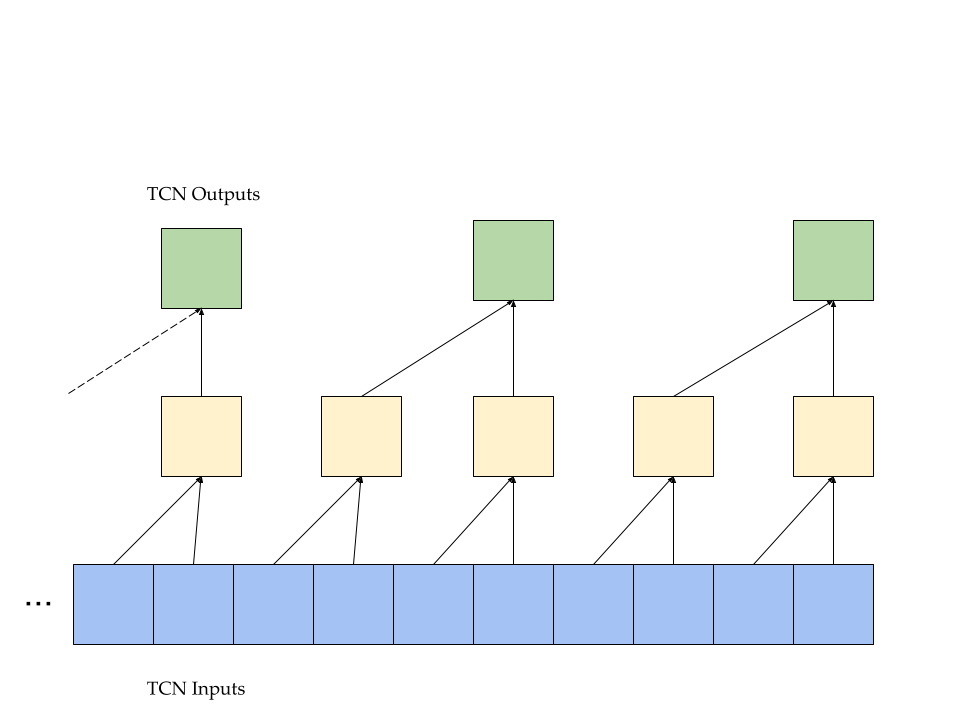
\includegraphics[width=13cm]{cap3/TCN.png}
    \caption[Temporal convolutional Network diagram]{Temporal Convolutional Network with output size 3 and two hidden layers each of dilatation factor 2}
    \label{fig:tcn}
\end{figure}

\section{Transformers}
\label{transformers_section}

\begin{figure}[h]
    \centering
    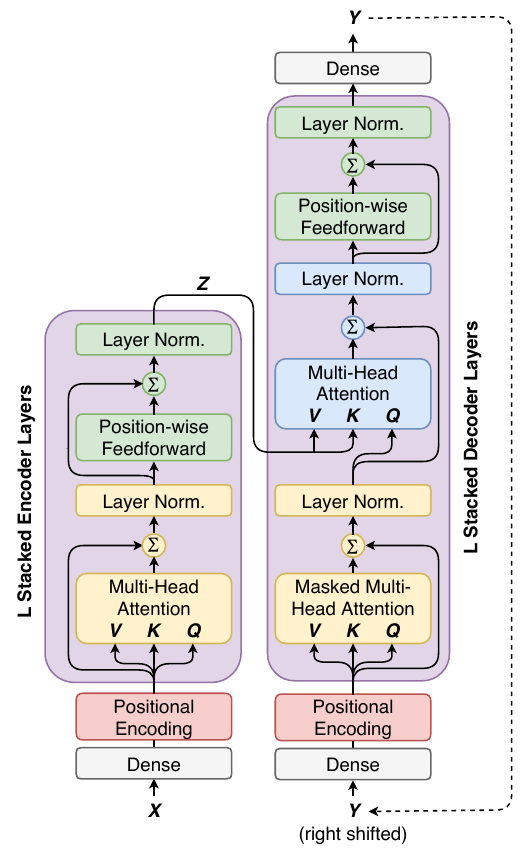
\includegraphics[width=8cm]{cap3/trasformers.png}
    \caption{Transformer architecture \cite{vaswani2017attention}}
    \label{fig:transformer_architecture}
\end{figure}



The Transformer neural model architecture, shown in figure \ref{fig:transformer_architecture}, was introduced by Vaswani et al. \cite{vaswani2017attention} in 2017 and at the time was the state of art in neural machine translation. Neural machine translation is the task where a machine translate from a language to another.

Compared to another typical architecture to deal with time series data, like the Long Short Term Memory network (LSTM) \cite{longshortterm},
Transformers do not compresses information as time goes by.
Such compression can weak long-distance relation patterns to some extent and may fail to highlight important information from historical data. Using \textbf{attention layers} (see section \ref{multi-head-attention}) it's possible to overcome this problem. Unlike previous sequence to sequence models, attention models do not process data sequentially but process all the sequence together. Attention layers learn temporal and spatial dependencies from the sequence. By processing all the sequence elements simultaneously, models that use attention are highly parallelizable and can take advantage of the computational power of GPU outclassing on performance LSTM. 

The transformer architecture follows a similar sequence-to-sequence/encoder decoder architecture. The encoder transformers an input sequence $X=[x_1,...,x_p]$ into a latent representation $Z=[z_1,...,z_m]$, and the decoder transforms $Z$ into an output sequence $Y=[y_1,...,y_r]$.  

The original Transformer was meant for language translation, a task where input data and output data have the same structure/typology, they are essentially phrases of a natural language. Our case is different, as in input we have different features derived from returns in the form of time series but output is a weight vector. This is the reason why in the original transformer shown in figure \ref{fig:transformer_architecture} the latent representation of $X$ is inserted in the middle of the decoder. The original transformer find matching between words of phrase $X$ and phrase $Y$, the essence of machine translation task, in their respective latent space. But as we are not doing machine translation, but regression, we remove the decoder part and we use the latent representation of $X$ namely $Z$ directly to compute the final network output through a Dense layer. We call this reduced architecture \textbf{Regression Transformer}. A representation of the regression Transformer can be see in figure \ref{fig:regression_transformer}.

\begin{figure}[h]
    \centering
    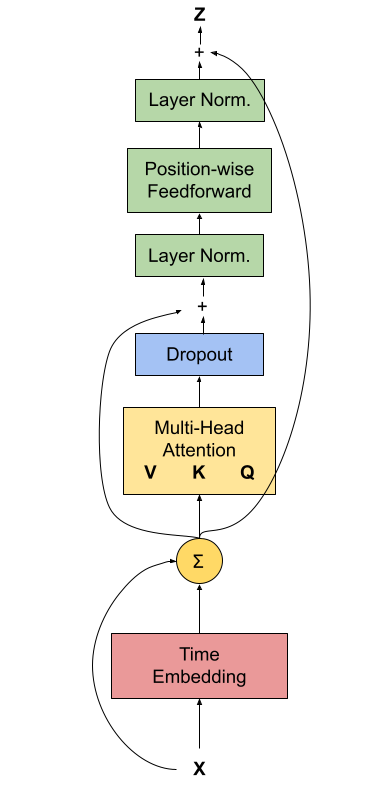
\includegraphics[width=6cm]{cap3/Regression_Transformer.png}
    \caption{Regression Transformer architecture}
    \label{fig:regression_transformer}
\end{figure}

\subsection{Time embedding}
For Attention to work, an encoding of time need to be attached to the input features. In the original NLP model, a collection of superimposed sinusoidal functions were added to each input embedding. We need a different representation as our inputs are scalar values and not distinct words/tokens.
Deep Neural Networks can learn linear and periodic components on their own, during training using a Time2Vec layer \cite{time2vec}.
Time2Vec is a learnable and complementary, model-agnostic representation of time. It decompose each input feature to a linear component and as many periodic (sinusoidal) components it's necessary. By defining the decomposition as a function, we can make the weights learnable through back propagation.
For a given scalar notion of time $\tau$, Time2Vec of $\tau$, denoted as $t2v(\tau)$, is a vector of size $k+1$ defined as follows:
$$ t2v(\tau)[i] = \begin{cases}
\omega_i \tau + \phi_i, & if \ i=0. \\
F(\omega_i \tau + \phi_i), & if \ 1 \leq i \leq k.
\end{cases}
$$
where $t2v(\tau)[i]$ is the $i$-th element of $t2v(\tau)$. $F$ is a periodic activation function, and $\omega_i$s and $\phi_i$s are learnable parameters. Given the prevalence of vector representation for different tasks, a vector representation for time makes it easily consumable by different architectures. We choose $F$ to be the sine function in our experiment.

The period of $\sin(\omega_i \tau + \phi)$ is $\frac{2 \pi}{\omega_i}$, i.e. it has the same value for $\tau$ and $\tau + \frac{2\pi}{\omega_i}$. Therefore, a since function helps capture period behavious without the need for feature engineering. For istance, a since function $sin(\omega \tau + \phi)$ with $\omega=\frac{2\phi}{7}$ repeats every 7 days (assuming $\tau$ indicates days) and can be potentially used to model weekly patterns.
The linear term represent the progression of time and can be used for capturing non-periodic patterns in the input that depend on time.


\subsection{Multi-head attention}
\label{multi-head-attention}
The primary innovation of the Transformer architecture is multi-head attention. Generic attention and dot-product attention will now be described as there are prerequisite to describing multi-head attention.

\hfill \break

An attention function can be described as mapping a query and a set of key-value pairs to an output where the query, keys, values and output are all vectors. The output is computed as a weighted sum of the values, where the weight assigned to each value is computed by a compatibility function of the query with the corresponding key. 

\hfill \break

In the \textit{scaled dot-product attention} the input consists of queries and keys of dimension $d_k$, and values of dimension $d_v$. The dot products of the query with all keys is computed. This dot product is divided by $\sqrt{d_k}$ to prevent the dot product from becoming large when $d_k$ is large as this may cause the softmax gradient to become very small and affect gradient descent training, and then a softmax function is applied to obtain the weight on the values. In practice, the attention function is computed on a set of queries simultaneously, packed together into a matrix Q. The keys and values are also packed together into matrices K and V. The matrix of output is computed as:
$$Attention(Q,K,V)=softmax\left( \frac{QK^T}{\sqrt{d_k}} \right )V$$

\hfill \break

\begin{figure}[h]
    \centering
    \subfloat[\centering Scaled dot product attention]{{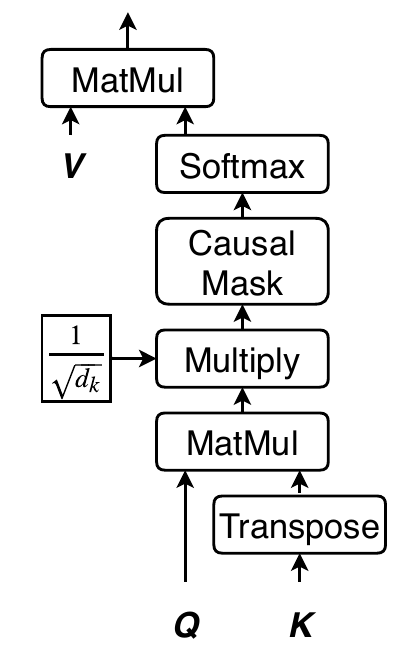
\includegraphics[width=0.3\textwidth]{cap3/scaled_dot_product_attention.png} }}%
    \qquad
    \subfloat[\centering Multi-head attention ]{{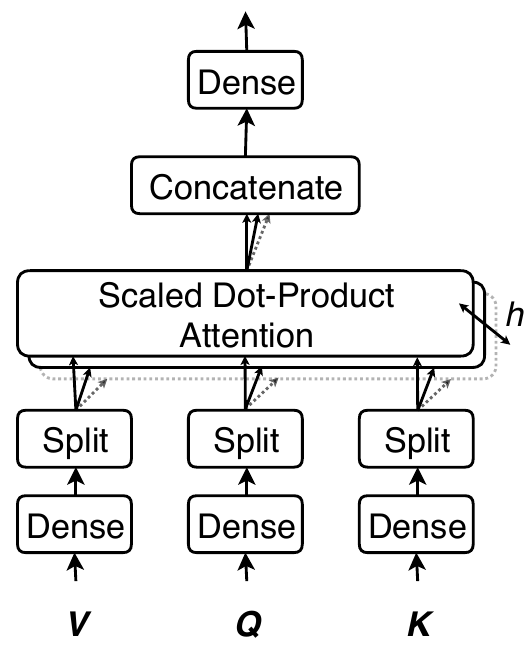
\includegraphics[width=0.3\textwidth]{cap3/multi-head-attention.png} }}%
    \caption[Fixed allocation anomaly]{Attention mechanism used in transformer architectures.}%
    \label{fig:attention_mechanisms}%
\end{figure}


Vasvani \cite{vaswani2017attention} also proposed multiheading shown in figure \ref{fig:attention_mechanisms} (b). It applies a separate dense layer to each of the values, queries and keys. The dense layer is applied with learned weight $W \in \mathbb{R}^{d \times d}$ and a learned bias vector $b \in \mathbb{R}^d$, where $d$ is the hidden dimension of the model, a hyperparameter. The outputs of the dense layers are then split along the last axis into $h$ sets, or heads. As a result the key, query and value dimension is reduced by a factor of $h$ to $\frac{d}{h}$. Scaled dot-product attention in then run independently on each set. The results are concatenated and put through a final dense layer to produce the output of the attention function. The dense layer function on the output has learned weights $W \in \mathbb{R}^{d \times d}$ and learned bias vector $b \in \mathbb{R}^{d \times d}$.

\hfill \break

The dense layer combined with the split allows the multi-head attention to pick out information from different subspaces in the input and direct these to different attention heads. This is in contrast to a single head which must average all subspaces.

\subsection{Residuals and Normalization}
Residual connections \cite{residual_connections} are applied around each sub-layer. That is, the output of each sub-layer is given by $X' = X + subLayer(X)$ where $subLayer(X)$ is the original output of the sub-layer. The outputs are then normalized by applying layer normalization \cite{layer_normalization}.

\section{Adam optimizer}
%TODO also add about clipnorm (also in chapter 4)
Adam is an algorithm for first-order gradient-based optimization of
stochastic objective functions, based on adaptive estimates of lower-order moments. It was introduced by P. Kingma in 2014 \cite{adam_optimizer}. The method computes individual adaptive learning rates for
different parameters from estimates of first and second moments of the gradients. The name Adam
is derived from adaptive moment estimation. Adam is designed to combine the advantages
of two other methods: AdaGrad, which works well with sparse gradients, and RMSProp, which works well in online and non-stationary
settings. For additional details and the presudocode of the method see the original paper \cite{adam_optimizer}.

\section{Errors and model capacity}
\label{s:errors_model_capacity}

In supervised machine learning we can divide the prediction error in 3 components \cite{bias_variance}: bias, variance and irreducible error:
$$E_m = E_b + E_v + E_i$$

Irreducible error is the error caused by the fact we do not have available all possible instances of the type of training data we use. For example if we want to build a classificator for bird species it would become a perfect classifier if we had all the possible pictures of birds to train with, but unfortunately is impossible. An example in finance would be that we do not have all possible market outcomes that can ever be possible in a stock exchange in the past and in the future. Generating them would be impossible because we do not know which future company would be in the market and how investors would react to it. This result in the fact that there is always a situation where the network is unprepared to deal with. Irreducible error can be very small, but it always exists.

\hfill \break

Model capacity is a measure of the ability of the model to learn complex functions from the data. Model capacity is the \textbf{dimension of the class $H$} to which the predictor $h_n$, described in the introduction of this chapter, belongs. Alternatively, but similarly, it can be defined as the number of parameters needed to define a function in the class $H$. Capacity is a trade-off, a medium point is preferable. Too high capacity leads to fitting the training data optimally, to have a small empirical risk but poor generalization on other datasets. This is the case of overfitting. Too low capacity and our model could not be able to learn the target function, to have a large empirical risk. This is the case of underfitting. The control of the function class capacity may be explicit, via the choice of $H$, for example by picking the neural network architecture, or it may be implicit, for example using regularization, for example internal parameters constraints. When a suitable balance is achieved, the performance of $h_n$, on the training data is said to generalize to the population $P$. 

\hfill \break

For example in k-nearest neighbors algorithm, the higher we set $k$ in the model, the lower is the capacity, the boundaries between classes are smoother and generalize better, until it reaches a point where boundaries are too simple and too many inputs are misclassified. Alternatively, with $k=1$ every point in the input is correctly classified in its class, but these boundaries fits very well the training dataset and only a slight variation of input characteristics in the validation datasets could lead to a high classification error. The model memorized the training dataset. Capacity is a characteristic of the architecture, not of the instanced model. The instanced model is characterized by its weight values and it can be overfitted or underfitted depending on how much it has been trained. Figure \ref{fig:bias_variance_training} show the relation between error rate, model capacity, bias, variance and irreducible error.

\begin{figure}[h]
    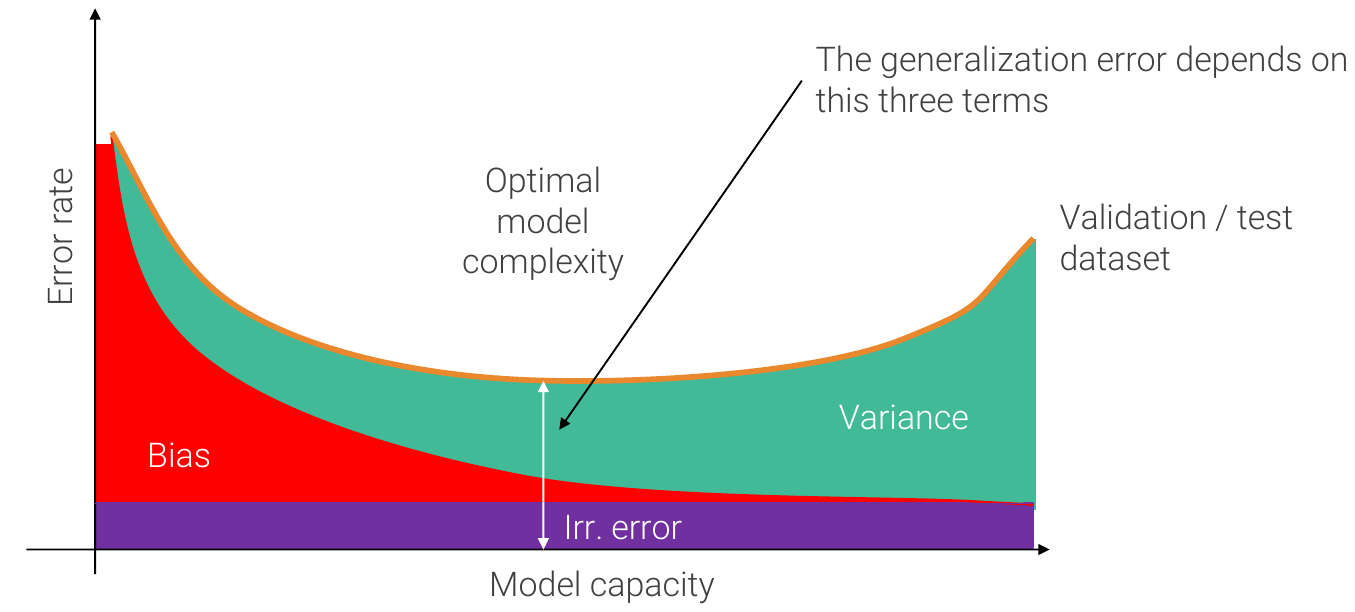
\includegraphics[width=13cm]{cap3/bias_variance_2.png}
    \caption[Bias, Variance and Irreducible error]{Bias-Variance-Irreducible error during training \cite{salti_cv} }  
    \label{fig:bias_variance_training}
\end{figure}



Given $n$ training/validation datasets, $n$ different models can be trained. Bias is the performance difference between model $i$ and the best model between the $n$. Variance is the difference between $i$ and the performance value average of  all the $n$ models.

\hfill \break

Another way to reduce variance, other than choosing a better model architecture or using more data, is regularization. Regularization is any modification we make to a training algorithm that is intended to reduce its generalization (test) error but not its training error. Examples of regularization are weight constraints, early stopping, dropout, etc...





